\documentclass{standalone}
\usepackage{tikz}
\usetikzlibrary{patterns, positioning}


\begin{document}
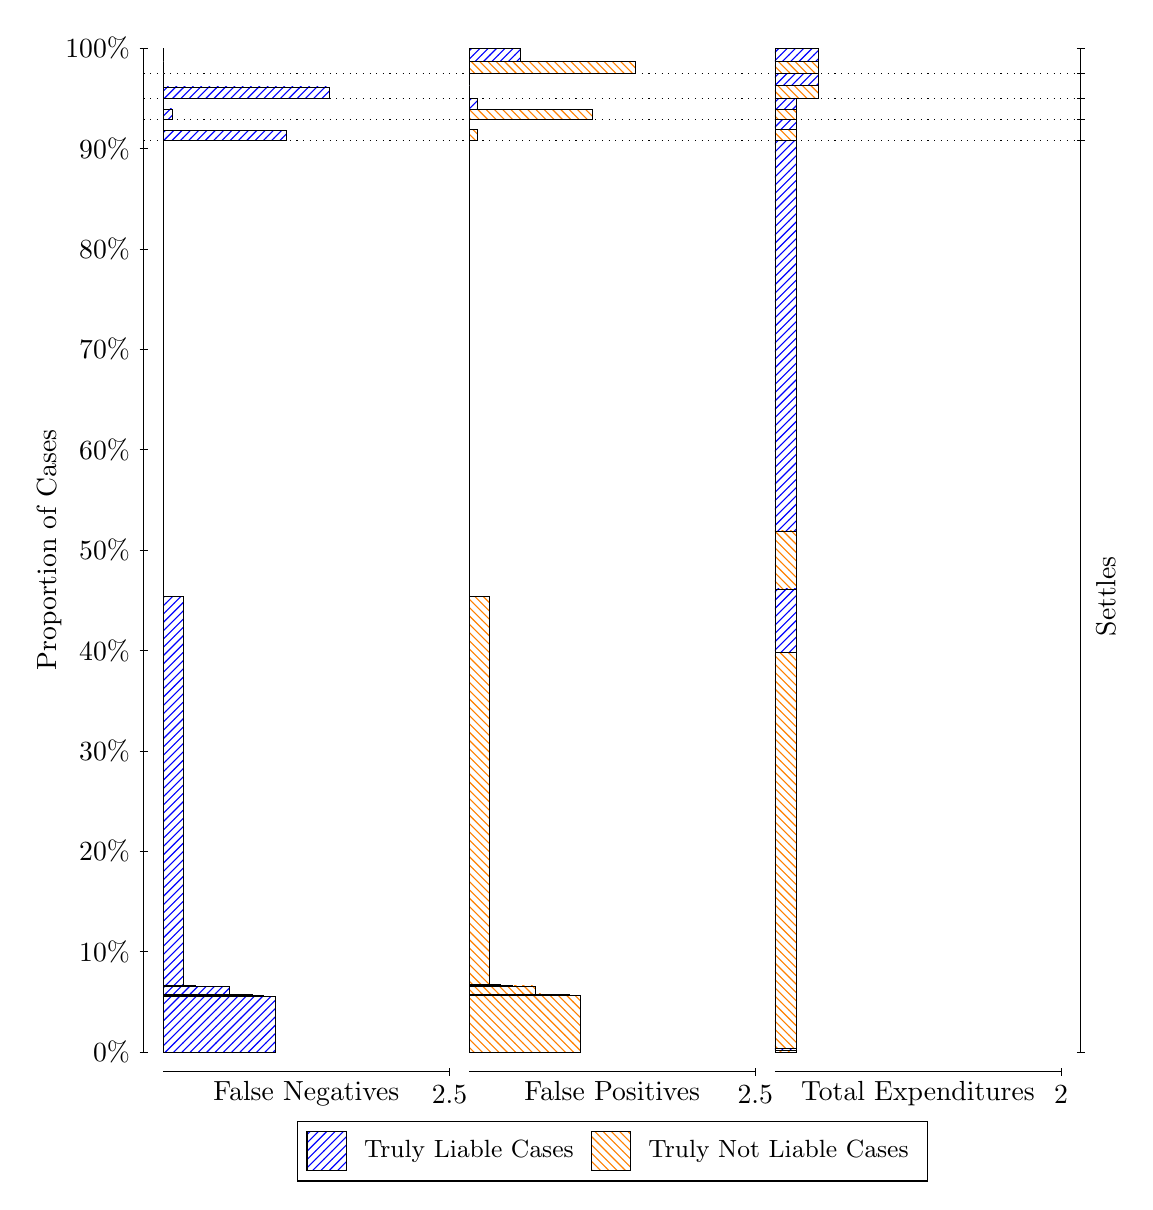
\begin{tikzpicture}
\draw[black, very thin] (1.5,1.75) -- (1.5,14.5);
\node[rotate=90, text=black, anchor=center] at (0.3, 8.125) {Proportion of Cases};
\draw[black, very thin] (1.45,1.75) -- (1.55,1.75);
\node[text=black, anchor=east] at (1.45, 1.75) {0\%};
\draw[black, very thin] (1.45,3.025) -- (1.55,3.025);
\node[text=black, anchor=east] at (1.45, 3.025) {10\%};
\draw[black, very thin] (1.45,4.3) -- (1.55,4.3);
\node[text=black, anchor=east] at (1.45, 4.3) {20\%};
\draw[black, very thin] (1.45,5.575) -- (1.55,5.575);
\node[text=black, anchor=east] at (1.45, 5.575) {30\%};
\draw[black, very thin] (1.45,6.85) -- (1.55,6.85);
\node[text=black, anchor=east] at (1.45, 6.85) {40\%};
\draw[black, very thin] (1.45,8.125) -- (1.55,8.125);
\node[text=black, anchor=east] at (1.45, 8.125) {50\%};
\draw[black, very thin] (1.45,9.4) -- (1.55,9.4);
\node[text=black, anchor=east] at (1.45, 9.4) {60\%};
\draw[black, very thin] (1.45,10.675) -- (1.55,10.675);
\node[text=black, anchor=east] at (1.45, 10.675) {70\%};
\draw[black, very thin] (1.45,11.95) -- (1.55,11.95);
\node[text=black, anchor=east] at (1.45, 11.95) {80\%};
\draw[black, very thin] (1.45,13.225) -- (1.55,13.225);
\node[text=black, anchor=east] at (1.45, 13.225) {90\%};
\draw[black, very thin] (1.45,14.5) -- (1.55,14.5);
\node[text=black, anchor=east] at (1.45, 14.5) {100\%};

\draw[black, very thin] (13.4,1.75) -- (13.4,14.5);
\draw[black, very thin] (13.35,1.75) -- (13.45,1.75);
\node[anchor=west] at (13.35, 1.75) {};
\draw[black, very thin] (13.35,13.326) -- (13.45,13.326);
\node[anchor=west] at (13.35, 13.326) {};
\draw[black, very thin] (13.35,13.59) -- (13.45,13.59);
\node[anchor=west] at (13.35, 13.59) {};
\draw[black, very thin] (13.35,13.856) -- (13.45,13.856);
\node[anchor=west] at (13.35, 13.856) {};
\draw[black, very thin] (13.35,14.178) -- (13.45,14.178);
\node[anchor=west] at (13.35, 14.178) {};
\draw[black, very thin] (13.35,14.5) -- (13.45,14.5);
\node[anchor=west] at (13.35, 14.5) {};

\draw[black, very thin, pattern color=blue, pattern=north east lines] (1.75,1.75) rectangle (3.167,2.4592);
\draw[black, very thin, pattern color=blue, pattern=north east lines] (1.75,2.4592) rectangle (3.0217,2.4734);
\draw[black, very thin, pattern color=blue, pattern=north east lines] (1.75,2.4734) rectangle (2.8763,2.4784);
\draw[black, very thin, pattern color=blue, pattern=north east lines] (1.75,2.4784) rectangle (2.731,2.48);
\draw[black, very thin, pattern color=blue, pattern=north east lines] (1.75,2.48) rectangle (2.5857,2.5805);
\draw[black, very thin, pattern color=blue, pattern=north east lines] (1.75,2.5805) rectangle (2.4403,2.5837);
\draw[black, very thin, pattern color=blue, pattern=north east lines] (1.75,2.5837) rectangle (2.295,2.5869);
\draw[black, very thin, pattern color=blue, pattern=north east lines] (1.75,2.5869) rectangle (2.1497,2.5971);
\draw[black, very thin, pattern color=blue, pattern=north east lines] (1.75,2.5971) rectangle (2.0043,7.538);
\draw[black, very thin, pattern color=orange, pattern=north west lines] (1.75,7.538) rectangle (1.75,13.326);
\draw[black, very thin, pattern color=blue, pattern=north east lines] (1.75,13.326) rectangle (3.3123,13.454);
\draw[black, very thin, pattern color=orange, pattern=north west lines] (1.75,13.454) rectangle (1.75,13.59);
\draw[black, very thin, pattern color=blue, pattern=north east lines] (1.75,13.59) rectangle (1.859,13.726);
\draw[black, very thin, pattern color=orange, pattern=north west lines] (1.75,13.726) rectangle (1.75,13.856);
\draw[black, very thin, pattern color=blue, pattern=north east lines] (1.75,13.856) rectangle (3.8573,14.007);
\draw[black, very thin, pattern color=orange, pattern=north west lines] (1.75,14.007) rectangle (1.75,14.178);
\draw[black, very thin, pattern color=orange, pattern=north west lines] (1.75,14.178) rectangle (1.75,14.33);
\draw[black, very thin, pattern color=blue, pattern=north east lines] (1.75,14.33) rectangle (1.75,14.5);
\draw[black, very thin, pattern color=orange, pattern=north west lines] (5.6333,1.75) rectangle (7.0503,2.4731);
\draw[black, very thin, pattern color=orange, pattern=north west lines] (5.6333,2.4731) rectangle (6.905,2.4822);
\draw[black, very thin, pattern color=orange, pattern=north west lines] (5.6333,2.4822) rectangle (6.7597,2.4852);
\draw[black, very thin, pattern color=orange, pattern=north west lines] (5.6333,2.4852) rectangle (6.6143,2.4881);
\draw[black, very thin, pattern color=orange, pattern=north west lines] (5.6333,2.4881) rectangle (6.469,2.5888);
\draw[black, very thin, pattern color=orange, pattern=north west lines] (5.6333,2.5888) rectangle (6.3237,2.5891);
\draw[black, very thin, pattern color=orange, pattern=north west lines] (5.6333,2.5891) rectangle (6.3237,2.5906);
\draw[black, very thin, pattern color=orange, pattern=north west lines] (5.6333,2.5906) rectangle (6.1783,2.5961);
\draw[black, very thin, pattern color=orange, pattern=north west lines] (5.6333,2.5961) rectangle (6.033,2.612);
\draw[black, very thin, pattern color=orange, pattern=north west lines] (5.6333,2.612) rectangle (5.8877,7.5377);
\draw[black, very thin, pattern color=blue, pattern=north east lines] (5.6333,7.5377) rectangle (5.6333,13.326);
\draw[black, very thin, pattern color=orange, pattern=north west lines] (5.6333,13.326) rectangle (5.7423,13.462);
\draw[black, very thin, pattern color=blue, pattern=north east lines] (5.6333,13.462) rectangle (5.6333,13.59);
\draw[black, very thin, pattern color=orange, pattern=north west lines] (5.6333,13.59) rectangle (7.1957,13.719);
\draw[black, very thin, pattern color=blue, pattern=north east lines] (5.6333,13.719) rectangle (5.7423,13.856);
\draw[black, very thin, pattern color=orange, pattern=north west lines] (5.6333,13.856) rectangle (5.6333,14.026);
\draw[black, very thin, pattern color=blue, pattern=north east lines] (5.6333,14.026) rectangle (5.6333,14.178);
\draw[black, very thin, pattern color=orange, pattern=north west lines] (5.6333,14.178) rectangle (7.7407,14.33);
\draw[black, very thin, pattern color=blue, pattern=north east lines] (5.6333,14.33) rectangle (6.2873,14.5);
\draw[black, very thin, pattern color=orange, pattern=north west lines] (9.5167,1.75) rectangle (9.7892,1.7732);
\draw[black, very thin, pattern color=blue, pattern=north east lines] (9.5167,1.7732) rectangle (9.7892,1.7939);
\draw[black, very thin, pattern color=orange, pattern=north west lines] (9.5167,1.7939) rectangle (9.7892,6.8204);
\draw[black, very thin, pattern color=blue, pattern=north east lines] (9.5167,6.8204) rectangle (9.7892,7.6301);
\draw[black, very thin, pattern color=orange, pattern=north west lines] (9.5167,7.6301) rectangle (9.7892,8.3682);
\draw[black, very thin, pattern color=blue, pattern=north east lines] (9.5167,8.3682) rectangle (9.7892,13.326);
\draw[black, very thin, pattern color=orange, pattern=north west lines] (9.5167,13.326) rectangle (9.7892,13.462);
\draw[black, very thin, pattern color=blue, pattern=north east lines] (9.5167,13.462) rectangle (9.7892,13.59);
\draw[black, very thin, pattern color=orange, pattern=north west lines] (9.5167,13.59) rectangle (9.7892,13.719);
\draw[black, very thin, pattern color=blue, pattern=north east lines] (9.5167,13.719) rectangle (9.7892,13.856);
\draw[black, very thin, pattern color=orange, pattern=north west lines] (9.5167,13.856) rectangle (10.062,14.026);
\draw[black, very thin, pattern color=blue, pattern=north east lines] (9.5167,14.026) rectangle (10.062,14.178);
\draw[black, very thin, pattern color=orange, pattern=north west lines] (9.5167,14.178) rectangle (10.062,14.33);
\draw[black, very thin, pattern color=blue, pattern=north east lines] (9.5167,14.33) rectangle (10.062,14.5);
\draw[black, dotted] (1.5,13.326) -- (13.4,13.326);
\draw[black, dotted] (1.5,13.59) -- (13.4,13.59);
\draw[black, dotted] (1.5,13.856) -- (13.4,13.856);
\draw[black, dotted] (1.5,14.178) -- (13.4,14.178);
\draw[black, very thin] (1.75,1.5) -- (5.3833,1.5);
\node[text=black, anchor=north] at (3.5667, 1.5) {False Negatives};
\draw[black, very thin] (5.3833,1.45) -- (5.3833,1.55);
\node[text=black, anchor=north] at (5.3833, 1.45) {2.5};

\draw[black, very thin] (5.6333,1.5) -- (9.2667,1.5);
\node[text=black, anchor=north] at (7.45, 1.5) {False Positives};
\draw[black, very thin] (9.2667,1.45) -- (9.2667,1.55);
\node[text=black, anchor=north] at (9.2667, 1.45) {2.5};

\draw[black, very thin] (9.5167,1.5) -- (13.15,1.5);
\node[text=black, anchor=north] at (11.333, 1.5) {Total Expenditures};
\draw[black, very thin] (13.15,1.45) -- (13.15,1.55);
\node[text=black, anchor=north] at (13.15, 1.45) {2};

\node[text=black, centered, rotate=90] at (13.72, 7.5378) {Settles};





\draw (7.449999999999999,1.5) node[draw=none] (baseCoordinate) {};
\begin{scope}[align=center]
        \matrix[scale=0.5, draw=black, below=0.5cm of baseCoordinate, nodes={draw}, column sep=0.1cm]{
            \node[rectangle, draw, minimum width=0.5cm, minimum height=0.5cm, pattern color=blue, pattern=north east lines] {}; &
            \node[draw=none, font=\small, text=black] (B) {Truly Liable Cases}; &
            \node[rectangle, draw, minimum width=0.5cm, minimum height=0.5cm, pattern color=orange, pattern=north west lines] {}; &
            \node[draw=none, font=\small, text=black] (B) {Truly Not Liable Cases}; \\
            };
\end{scope}

\end{tikzpicture}
\end{document}